\subsection{Decision Trees}

	Decision trees are applied to both, classification and regression.	
	\todo{Chapter 11}

	\subsubsection{Classification Trees}	
		\paragraph{Binary Splitting}
			In binary splitting, a training set is used to split up the predictor domain into regions which contain data for which the response variable belongs to the same class. By \textbf{binary} it is meant that a region is split into \textbf{two} subregions (i.e. ``is a predictor less or greater than a threshold value?'' \textrightarrow\ yes/no).
			
			\RTheory
			{%
				\textbf{Algorithm:}
				\begin{enumerate}
				  	\item Initialise the set of regions $\mathcal{R} = {R}$ by the predictor domain $R$
				  	\item\label{itm:binarySplitStart}  Choose the optimal region $R$ in $\mathcal{R}$ and the optimal predictor $X_i$ such that a binary split of $R$ with respect to $X$
						$$R_1 = \{\vec{x} \in R | x_i > t\} \quad\mathrm{and}\quad R_2 = \{\vec{x} \in R | x_i \leq t\}$$
						gives the highest gain in purity (for some threshold $t$).
					\item Replace $R$ in $\mathcal{R}$ with $R_1$ and $R_2$ and return to \ref{itm:binarySplitStart}.
				\end{enumerate}
				
				The iteration is stopped if the current splitting fulfils a pre-defined stopping criterion.
				
			}
			{
				sections/Classification/DecisionTrees/BinarySplitting/theoryExample.R
			}
			
			\begin{figure}[H]\centering
			    \begin{subfigure}[b]{0.3\textwidth}
			        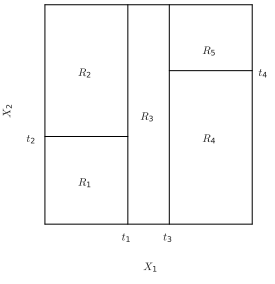
\includegraphics[width=\textwidth]{sections/Classification/DecisionTrees/BinarySplitting/binarySplittingRegions.png}
			        \caption{Example regions resulting from binary splitting}
			        \label{fig:binarySplittingRegions}
			    \end{subfigure}
			    \hspace{0.5cm}
			    \begin{subfigure}[b]{0.3\textwidth}
			        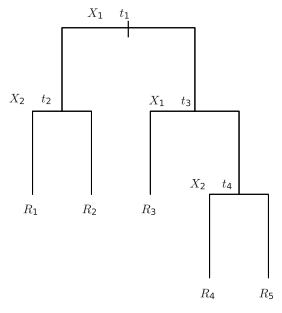
\includegraphics[width=\textwidth]{sections/Classification/DecisionTrees/BinarySplitting/binarySplittingTree.png}
			        \caption{Example decision tree resulting from binary splitting}
			        \label{fig:binarySplittingTree}
			    \end{subfigure}
			\end{figure}
			
		\paragraph{Node Purity}
			\textbf{Notation:}
			\begin{twoColTable}
				\hline
				\twoColHdrCell{Variable} & \twoColHdrCell{Description}\\
				\hline
				$Y$						& Response variable\\
				\hline
				$K$						& Levels (categories) of the response variable\\
				\hline
				$T$						& The decision tree\\
				\hline
				$M$						& Amount of terminal nodes\\
				\hline
				$\hat{p}_{mk}$			& proportion of the training data in region $m$ from level $k$\\
				\hline 
			\end{twoColTable}
			
			\textbf{Purity Measures:}
			{
				\setlength{\extrarowheight}{4pt}
				\begin{twoColTable}
					\hline
					Classification error rate	& $E_m(T) = 1 - \max\limits_k(\hat{p}_{mk})$\\
					\hline
					Gini index					& $G_m(T) = \sum\limits_{k=1}^{K}\hat{p}_{mk}\cdot(1-\hat{p}_{mk})$\\
					\hline
					Cross-entropy				& $D_m(T) = -\sum\limits_{k=1}^{K}\hat{p}_{mk}\cdot\log(\hat{p}_{mk})$\\
					\hline
				\end{twoColTable}
			}
			
			\RCode%
			{%
				Cross Entropy and Gini measures in R%
			}%
			{%
				sections/Classification/DecisionTrees/NodePurity/CrossEntropyGiniExample.R%
			}
			
		\paragraph{Making Predictions}
			\RExample
				{
					sections/Classification/DecisionTrees/MakingPredictions/sourceCode.R
				}
				{
					sections/Classification/DecisionTrees/MakingPredictions/output.R
				}
				{
					\todo{Interpretation here}
				}
				
		\paragraph{Tree Pruning}
		    Tree Pruning is the process of reducing the number of tree nodes based on various techniques.
			This is done in order to reduce the size of the mode, because, for example, smaller models usually generalize better and may take less computing time.
			
			\subparagraph{Cost Complexity Pruning}
				\begin{twoColTable}
					\hline
					\twoColHdrRow{General Definitons}\\
					\endhead
					\hline
					Number of terminal nodes
						& $|T|$\\
					\hline
					Number of elements in the node
						& $N_m$\\
					\hline
					Arbitrary node purity measure (e.g. Gini Index)
						& $Q_m(T)$\\
					\hline
					Cost-Complexity Function of subtree $T$
						& $R_\alpha(T) = \sum\limits_{m=1}^{|T|} N_m Q_m(T) + \alpha|T|, \qquad \alpha \geq 0$\\
					\hline
				\end{twoColTable}
				
				\RTheory
				{
					\begin{enumerate}
					    \item Use recursive binary splitting to grow a very large tree $T_0$ and set $\alpha = 0$
					    \item Increase $\alpha$ and for each value compute the subtree $T_\alpha$ that minimizes the cost-complexity function $R_\alpha(T)$
					    \item Stop if $T_\alpha$ is the root node
					\end{enumerate}
				}
				{
					sections/Classification/DecisionTrees/TreePruning/CostComplexityExample.R
				}
			
			
			
			